% ============================================================
% A4 Landscape Exam Cheat Sheet Template
% 4 columns per page, 2 pages (i.e. 8 columns total)
% ============================================================
\documentclass[10pt]{extarticle}

% ---------- Page geometry: A4 landscape, tight margins ----------
\usepackage[a4paper, landscape, margin=0.4cm]{geometry}

\usepackage{tikz}
\usetikzlibrary{arrows.meta, positioning}

\usepackage{amsmath}
\usepackage{array}
\usepackage{multirow}
\usepackage{bigdelim}

\usepackage{graphicx}
\usepackage{mathtools}

% ---------- Multi-column layout ----------
\usepackage{multicol}
\setlength{\columnsep}{0.5cm}
\setlength{\columnseprule}{0.4pt}

% ---------- Fonts & sizing ----------
\usepackage[utf8]{inputenc}
\usepackage[T1]{fontenc}
\renewcommand{\familydefault}{\sfdefault}

% ---------- Math ----------
\usepackage{amsmath, amssymb, amsthm}

% ---------- Compact spacing ----------
\usepackage{titlesec}
\usepackage{enumitem}
\setlist{nosep, leftmargin=1.1em, itemsep=0pt, parsep=0pt, topsep=1pt}

% Compact section headers
\titleformat{\section}
  {\normalfont\bfseries\small\color{black}}
  {}{0em}{}
\titlespacing{\section}{0pt}{4pt}{2pt}

\titleformat{\subsection}
  {\normalfont\bfseries\footnotesize}
  {}{0em}{}
\titlespacing{\subsection}{0pt}{3pt}{1pt}

% ---------- Misc useful packages ----------
\usepackage{graphicx}
\usepackage{array}
\usepackage{booktabs}
\usepackage{xcolor}
\usepackage{tcolorbox}
\tcbuselibrary{skins, breakable}

% Remove page numbers / headers footers to save space
\usepackage{fancyhdr}
\pagestyle{empty}

% Zero out paragraph indent/skip to save vertical space
\setlength{\parindent}{0pt}
\setlength{\parskip}{0pt}

% Tiny custom box for formulas / key results
\newtcolorbox{formulabox}[1][]{
  colback=gray!5, colframe=black!60,
  boxrule=0.3pt, arc=1pt,
  left=2pt, right=2pt, top=1pt, bottom=1pt,
  #1
}

% Shortcut for a compact rule under section titles
\newcommand{\sectionrule}{\vspace{-2pt}\hrule\vspace{2pt}}

% Helper macros for drawing kernel grids
\newcommand{\kernelrow}[3]{%
\begin{tabular}{|c|c|c|}
\hline #1 & #2 & #3 \\
\hline
\end{tabular}}

\newcommand{\kernelgrid}[9]{%
\begin{tabular}{|c|c|c|}
\hline #1 & #2 & #3 \\
\hline #4 & #5 & #6 \\
\hline #7 & #8 & #9 \\
\hline
\end{tabular}}

\begin{document}
\footnotesize % base font size for body text; tune to 8pt/9pt/tiny as needed

% ============================================================
% PAGE 1 — 4 columns
% ============================================================
\begin{multicols}{4}
\begin{center}
  {\Large\bfseries CS4243 Cheatsheet}\\[2pt]
  Emilia Ayu
  \rule{\linewidth}{0.6pt}
\end{center}
\vspace{-1.5em}
\section*{Variables and Operations}
\subsection*{Statistics}
\begin{description}[leftmargin=1.4em, itemsep=1pt]
  \item[Mean / Std. dev.] \hfill \\[0.3em]
  \begin{minipage}[t]{0.48\linewidth}
    $\bar{x} = \dfrac{1}{n}\sum_{i=1}^n x_i$
  \end{minipage}%
  \begin{minipage}[t]{0.48\linewidth}
    $\sigma = \sqrt{\dfrac{1}{n}\sum_i (x_i-\bar x)^2}$
  \end{minipage}
  \item[Normalisation] \mbox{$x' = \dfrac{x-\mu}{\sigma}$ \; (or min-max: $\dfrac{x-\min}{\max-\min}$)}
  \item[Gaussian (1D)] $G(x) = \dfrac{1}{\sqrt{2\pi}\,\sigma}\,e^{-x^2/2\sigma^2}$
  \item[Gaussian (2D)] $G(x,y) = \dfrac{1}{2\pi\sigma^2}\,e^{-(x^2+y^2)/2\sigma^2}$
\end{description}

\resizebox{\linewidth}{!}{%
\begin{tabular}{@{}ll@{}}
\textbf{Accuracy:} $\dfrac{TP+TN}{TP+TN+FP+FN}$ & \textbf{Precision:} $\dfrac{TP}{TP+FP}$ \\[6pt]
\textbf{Recall:} $\dfrac{TP}{TP+FN}$ & \textbf{F1-score:} $\dfrac{2\,P\,R}{P+R}$
\end{tabular}}

\subsection*{Calculus}
\resizebox{\linewidth}{!}{%
\begin{tabular}{@{}ll@{}}
\textbf{Line eqns:} $y=mx+b$; \newline $x\cos\theta+y\sin\theta=\rho$
&
\textbf{Euclidean dist:} $d=\sqrt{\sum_i(x_i-y_i)^2}$
\\[6pt]
\textbf{Gradient:} $\nabla f=\left(\dfrac{\partial f}{\partial x},\dfrac{\partial f}{\partial y}\right)$
&
\textbf{Laplacian:} $\nabla^2 f=\dfrac{\partial^2 f}{\partial x^2}+\dfrac{\partial^2 f}{\partial y^2}$
\\[6pt]
\textbf{Orientation:} $\theta=\tan^{-1}\!\left(\dfrac{f_y}{f_x}\right)$
&
\textbf{Magnitude:} $\|\nabla f\|=\sqrt{f_x^2+f_y^2}$
\end{tabular}}


\section*{Lecture 1 - Computer Vision}
\sectionrule


\textbf{Digital Image Acquisition}

\vspace{0.5em}

\textbf{Illuminance} ($i(x,y)$, $0 \leq i \leq \infty$): amount of source illumination incident on scene.\\
\textbf{Reflectance} ($r(x,y)$, $0 \leq r \leq 1$): amount of source illumination reflected by objects on scene.

\textbf{Exposure}: amount of time incident light can reach imaging sensor. \\
\textbf{Aperture}: how much light you let in (too much: bokeh, too narrow sharp image\\
\textbf{Shutter Speed}: how much time you give light to accumulate (slow: motion blur, fast: freeze action)

\vspace{-1.5em}

\begin{center}
    \small
    {\tiny
    \begin{tabular}{|p{1.5cm}|p{2cm}|p{2cm}|}
        \hline
        & \textbf{Spatial Resolution} & \textbf{Intensity Resolution} \\
        \hline
        Definition & smallest discernible detail & smallest discernible $\delta$ intensity level \\
        \hline
        Measurement & pixels / unit distance & bit depth / pixel value \\
        \hline
        Determined by & sampling & quantisation \\
        \hline
        Effects of low res & pixellation & false contouring \\
        \hline
    \end{tabular}
    }
    \label{tab:spatial-intensity}
\end{center}
\vspace{-1.5em}

\textbf{File size (bits)}: $b = M \cdot N \cdot k$ \\
\footnotesize
$M$: rows, $N$: columns, $k$: bits/pixel, $b$: total bits

\subsection{File Extensions}
\textbf{.bmp}: raw bit file (largest size) \\
\textbf{.png}: predicts pixels based on neighbours, reconstructs original pixel value (lossless) \\
\textbf{.jpg}: 8x8 image blocks represented by 64 Discrete Cosine Transform coefficients, reconstruction is approximate (lossy). Zigzag ordering captures larger coefficients first; more efficient for Huffman entropy encoding

\subsection{Colour Representation}
\textbf{RGB Space}
$im(x, y, b)$ = $y$ pixels down, $x$ pixels to right in the $b$th channel \\
\textbf{HSV Space} Hue Saturation Value

\subsection{Bayer Filter}
Each pixel only stores one color sample over it (RGB). Reduces intensity resolution.
\begin{center}
    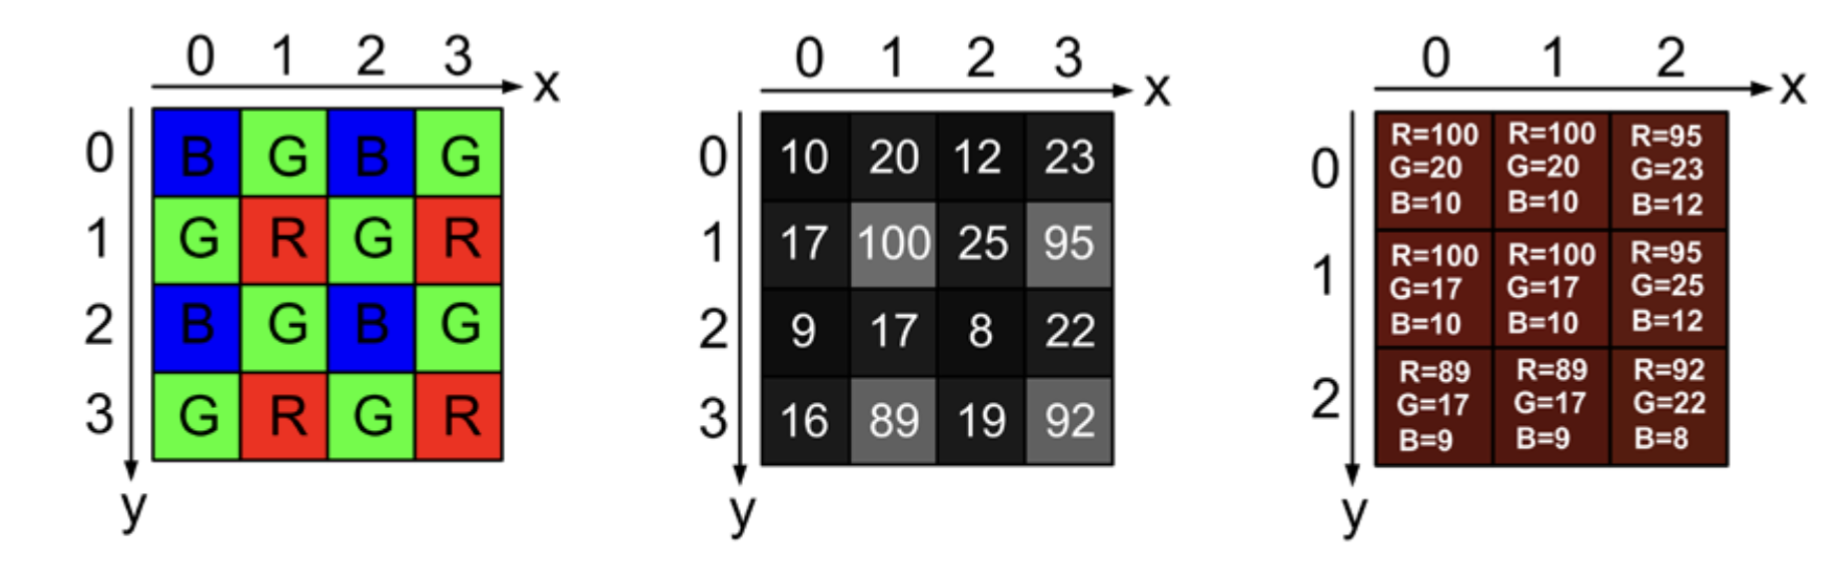
\includegraphics[width=0.5\linewidth]{demosaic.png}
\end{center}
\vspace{-2.0em}
\begin{center}
    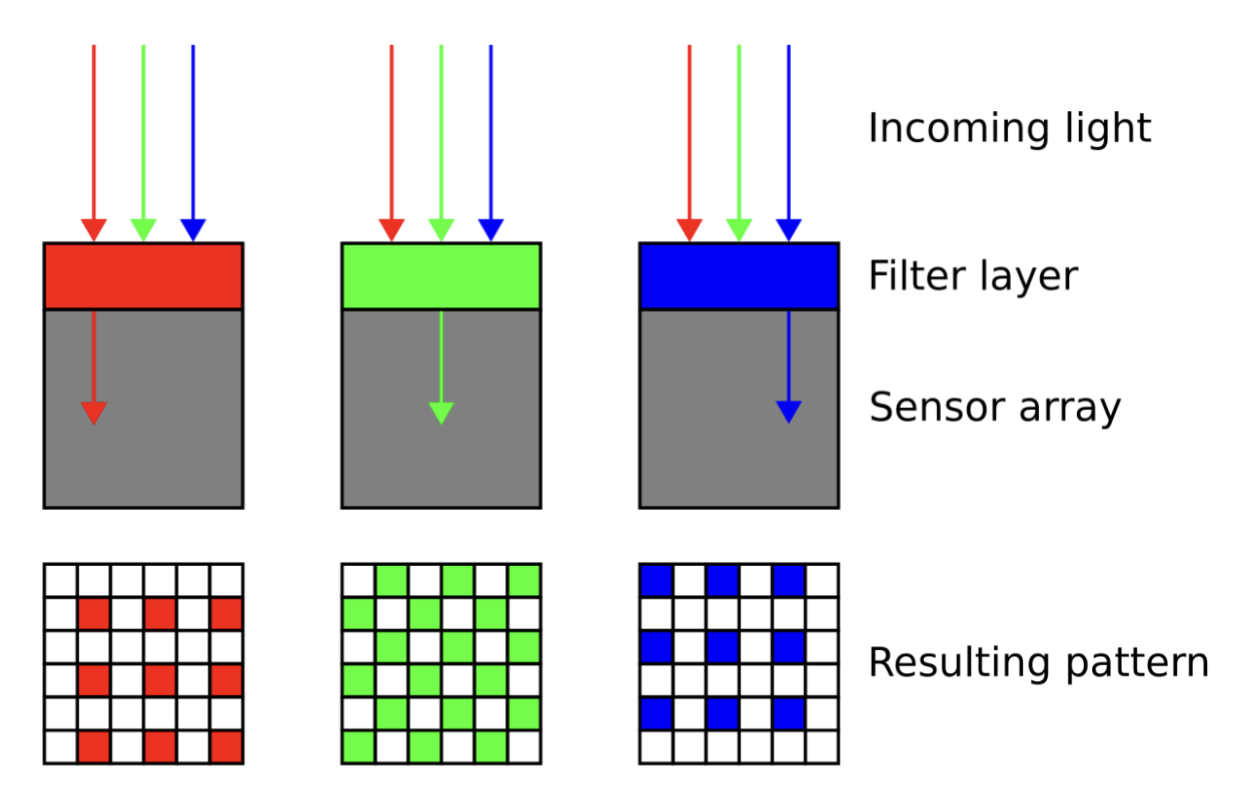
\includegraphics[width=0.5\linewidth]{bayer.png}
\end{center}

\resizebox{\linewidth}{!}{%
\begin{tabular}{c c l c l}
\multirow{4}{*}{$g(x,y)$} & \ldelim\{{4}{0pt} & $[R,G,B]_B = [f(x+1,y+1), f(x+1,y), f(x,y)]$ & & \text{sensitive to blue} \\[6pt]
 & & $[R,G,B]_{GB} = [f(x,y+1), f(x,y), f(x-1,y)]$ & \multirow{2}{*}{\rdelim\}{2}{0pt}} & \text{sensitive to green followed by} \\
 & & $[R,G,B]_{GR} = [f(x+1,y), f(x,y), f(x,y-1)]$ & & \text{blue / red in row} \\[6pt]
 & & $[R,G,B]_{R} = [f(x,y), f(x-1,y), f(x-1,y-1)]$ & & \text{sensitive to red} \\
\end{tabular}}


\section*{Lecture 2 - Point Processing and Filtering}
\sectionrule
\textbf{Point processing: } $x_{ij} = f(p_{ij})$ \\
\textbf{Filtering: } $x_{ij} = f(w_{ij})$ 

\subsection{Point Processing}
Brightness = $x_{ij} = p_{ij} + b$ (clip when needed) \\
Intensity scaling = $x_{ij} = a \cdot p_{ij}$

\textbf{Image Standardisation} Preprocess to remove arbitrary brightness/contrast baselines. Algorithms process better when inputs are centered around 0.

\textbf{Histogram Stretching vs. Equalisation}
\begin{center}
    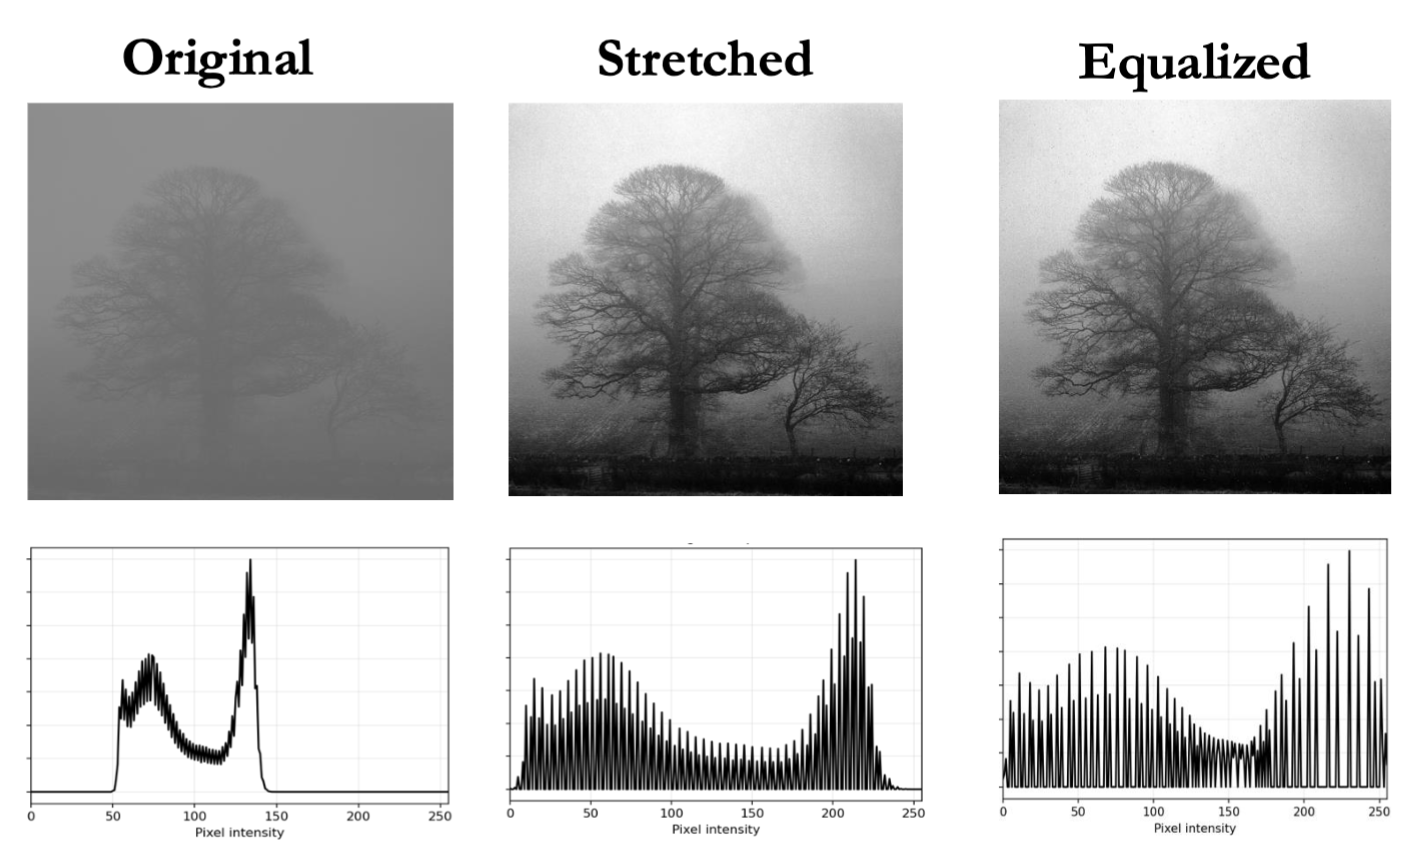
\includegraphics[width=0.5\linewidth]{histogram.png}
\end{center}
\textbf{Stretching:} linear rescale to full range
$$s = \frac{r-r_{\min}}{r_{\max}-r_{\min}}(L-1)$$
\textbf{Pros:} improves contrast; preserves relative brightness relationships \\
\textbf{Cons:} limited effect if histogram already spans most of the range

\textbf{Equalisation:} redistribute via CDF for uniform histogram
$$s = (L-1)\sum_{k=0}^{r} p(k), \quad s_{output} = k \cdot CDF(s_{input})$$
\textbf{Pros:} more dramatic contrast change; reveals poorly represented ranges automatically \\
\textbf{Cons:} can amplify noise; alters clinically irrelevant contrast

\subsection{Cross-Correlation and Convolution}

\textbf{Purpose:} smoothing/averaging with neighbours reduces impulse (salt-and-pepper) noise; also used for edge detection and template matching. \\
\textbf{Cross-Correlation:} slide kernel $F$ as-is, multiply \& sum
$$x_{ij} = \sum_{u}\sum_{v} f_{uv} \cdot p_{i+u,\,j+v}, \qquad X = P \circledast F$$
\textbf{Convolution:} flip kernel $180^\circ$ first, then multiply \& sum. Commutative and associative.
$$x_{ij} = \sum_{u}\sum_{v} f_{uv} \cdot p_{i-u,\,j-v}, \qquad X = P * F$$
\textbf{Equal when:} kernel is symmetric under $180^\circ$ rotation, i.e.\ $F = F_{flip}$ (e.g.\ box filter, Gaussian). 

\textbf{Gaussian Kernel}\\
Used as the filter $f_{uv}$ in cross-correlation/convolution above to smooth/blur.
Larger $\sigma$ = more blur.

\vspace{4pt}
\textbf{Detail extraction (unsharp masking):}\\
$\text{Details} = \text{Original} - \text{Blurred}$
\quad $\Rightarrow$ \quad
$\text{Sharpened} = \text{Original} + \alpha\cdot\text{Details}$

\section*{Lecture 3 - Gradients}
\sectionrule
\subsection{Sobel Filter}
\begin{center}
    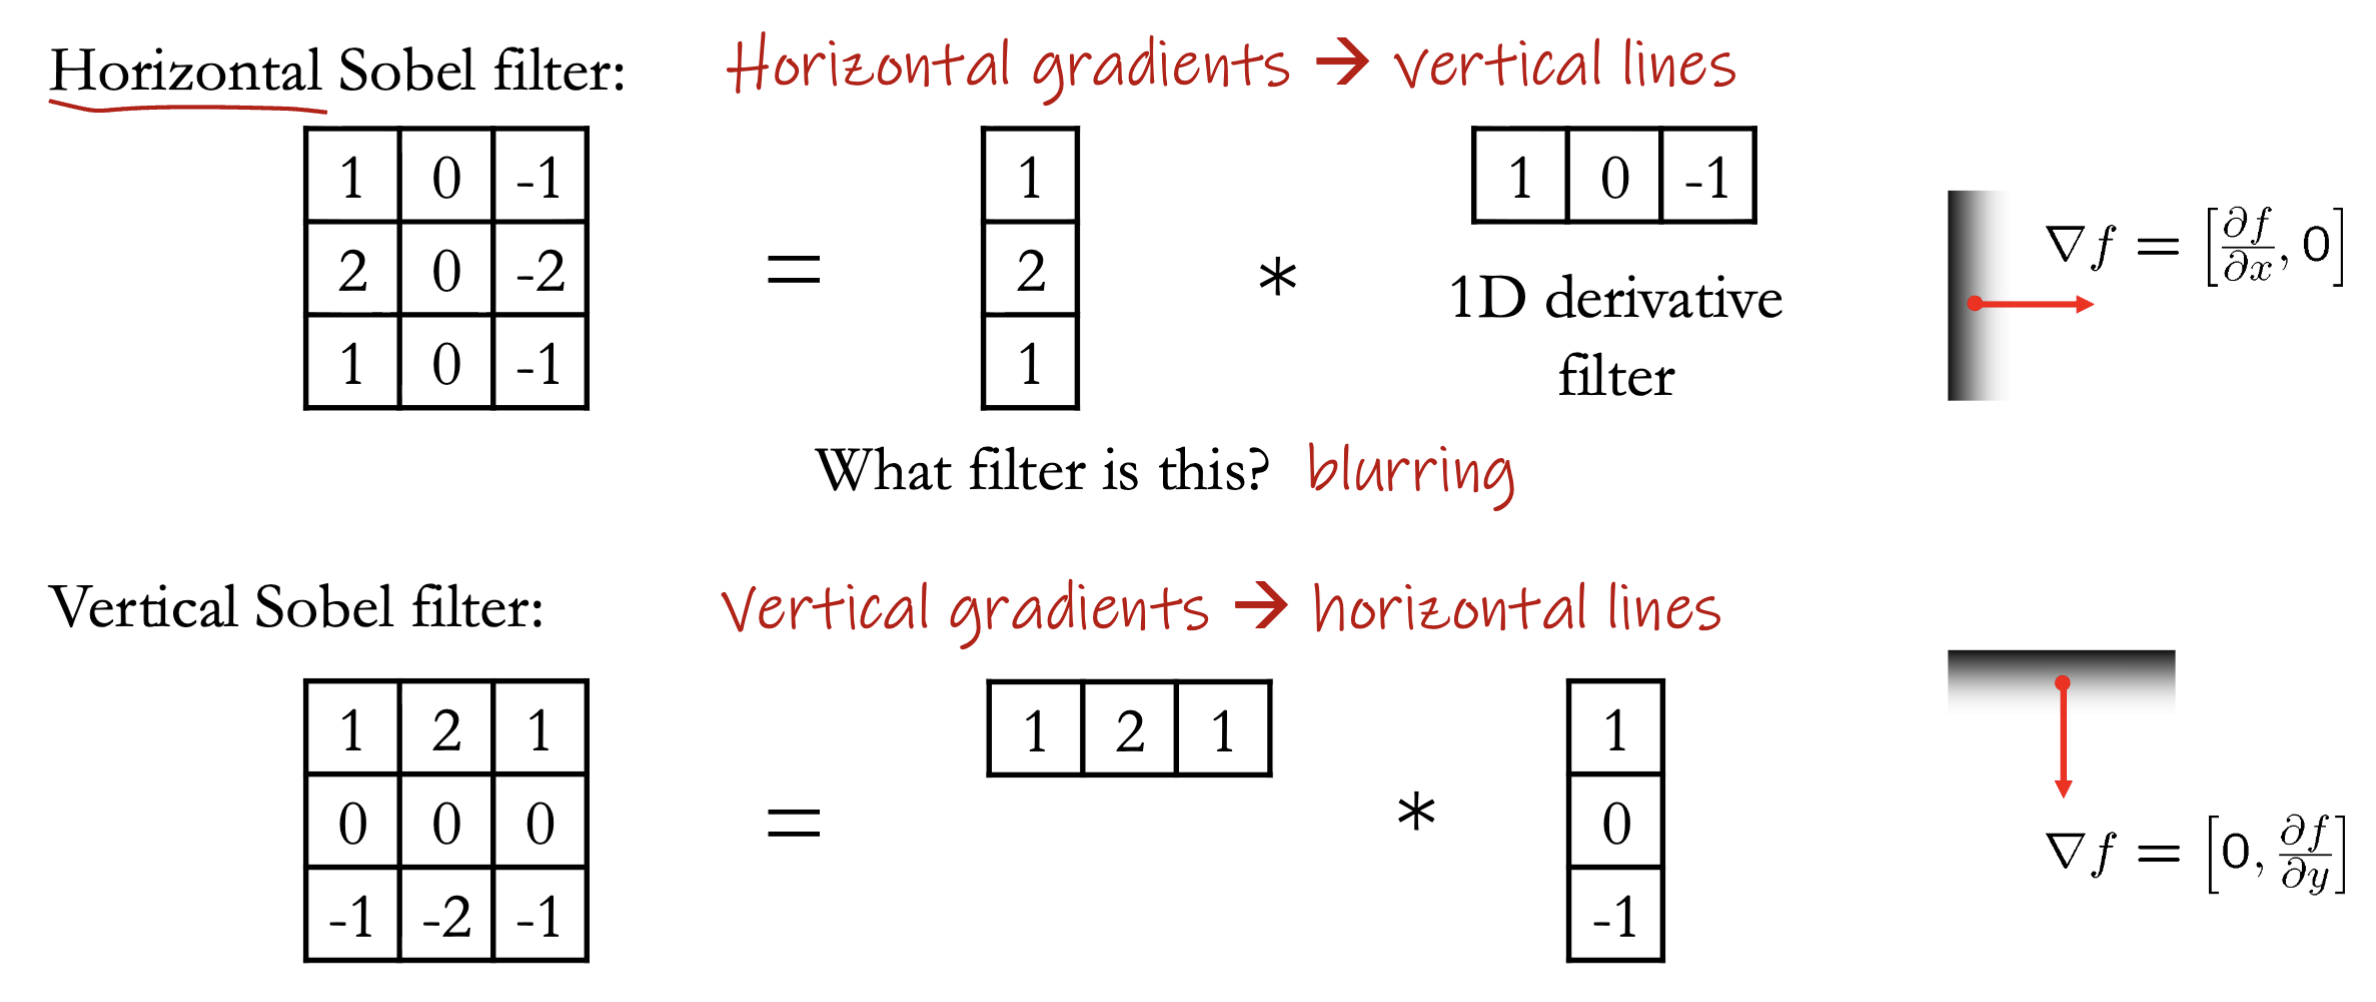
\includegraphics[width=0.75\linewidth]{sobel-1.png}
\end{center}

Vertical filter $S_y$ detects horizontal edges; 
horizontal filter $S_x$ detects vertical edges (both across gradient). \\
The gradient points across the edge, ie direction is normal to the edge. Gradient will point from darker to brighter intensities. The edge occurs at peaks.

A 2D filter is \textbf{separable} if it can be written as an outer product of a
column vector and a row vector:
$$K = u\,v^T$$
Convolving with the full 2D kernel $K$ is equivalent to convolving with $u$ then $v$
separately. Cheaper since $1\times n + n\times 1$ multiplications beat $n\times n$.

\vspace{4pt}
\textbf{Example — Vertical Sobel filter:}
\begin{enumerate}[leftmargin=1.2em, itemsep=1pt]
  \item \textbf{Smooth} horizontally: $[1,\,2,\,1]$
  \item \textbf{Differentiate} vertically: $[1,\,0,\,-1]^T$
\end{enumerate}
$$S_y = \begin{bmatrix}1\\0\\-1\end{bmatrix}\begin{bmatrix}1 & 2 & 1\end{bmatrix}$$

\textbf{Computing gradients}
\begin{enumerate}
    \item Convolve gradient filter with image f to compute image gradient components \\ 
    $\mathbf{G_x} = \dfrac{\partial \boldsymbol{f}}{\partial x} = \boldsymbol{S}_x * \boldsymbol{f}$
    \qquad
    $\mathbf{G_y} = \dfrac{\partial \boldsymbol{f}}{\partial y} = \boldsymbol{S}_y * \boldsymbol{f}$
    \item Compute gradient orientation and magnitude
\end{enumerate}

\subsection{Gaussian Derivative and Laplace Filters}
Differentiation accentuates noise (multiplicative factor proportional to frequency) $\Rightarrow$ blur before using derivative features to remove noise (but the edge will blur).
\vspace{-1.5em}
\begin{center}
    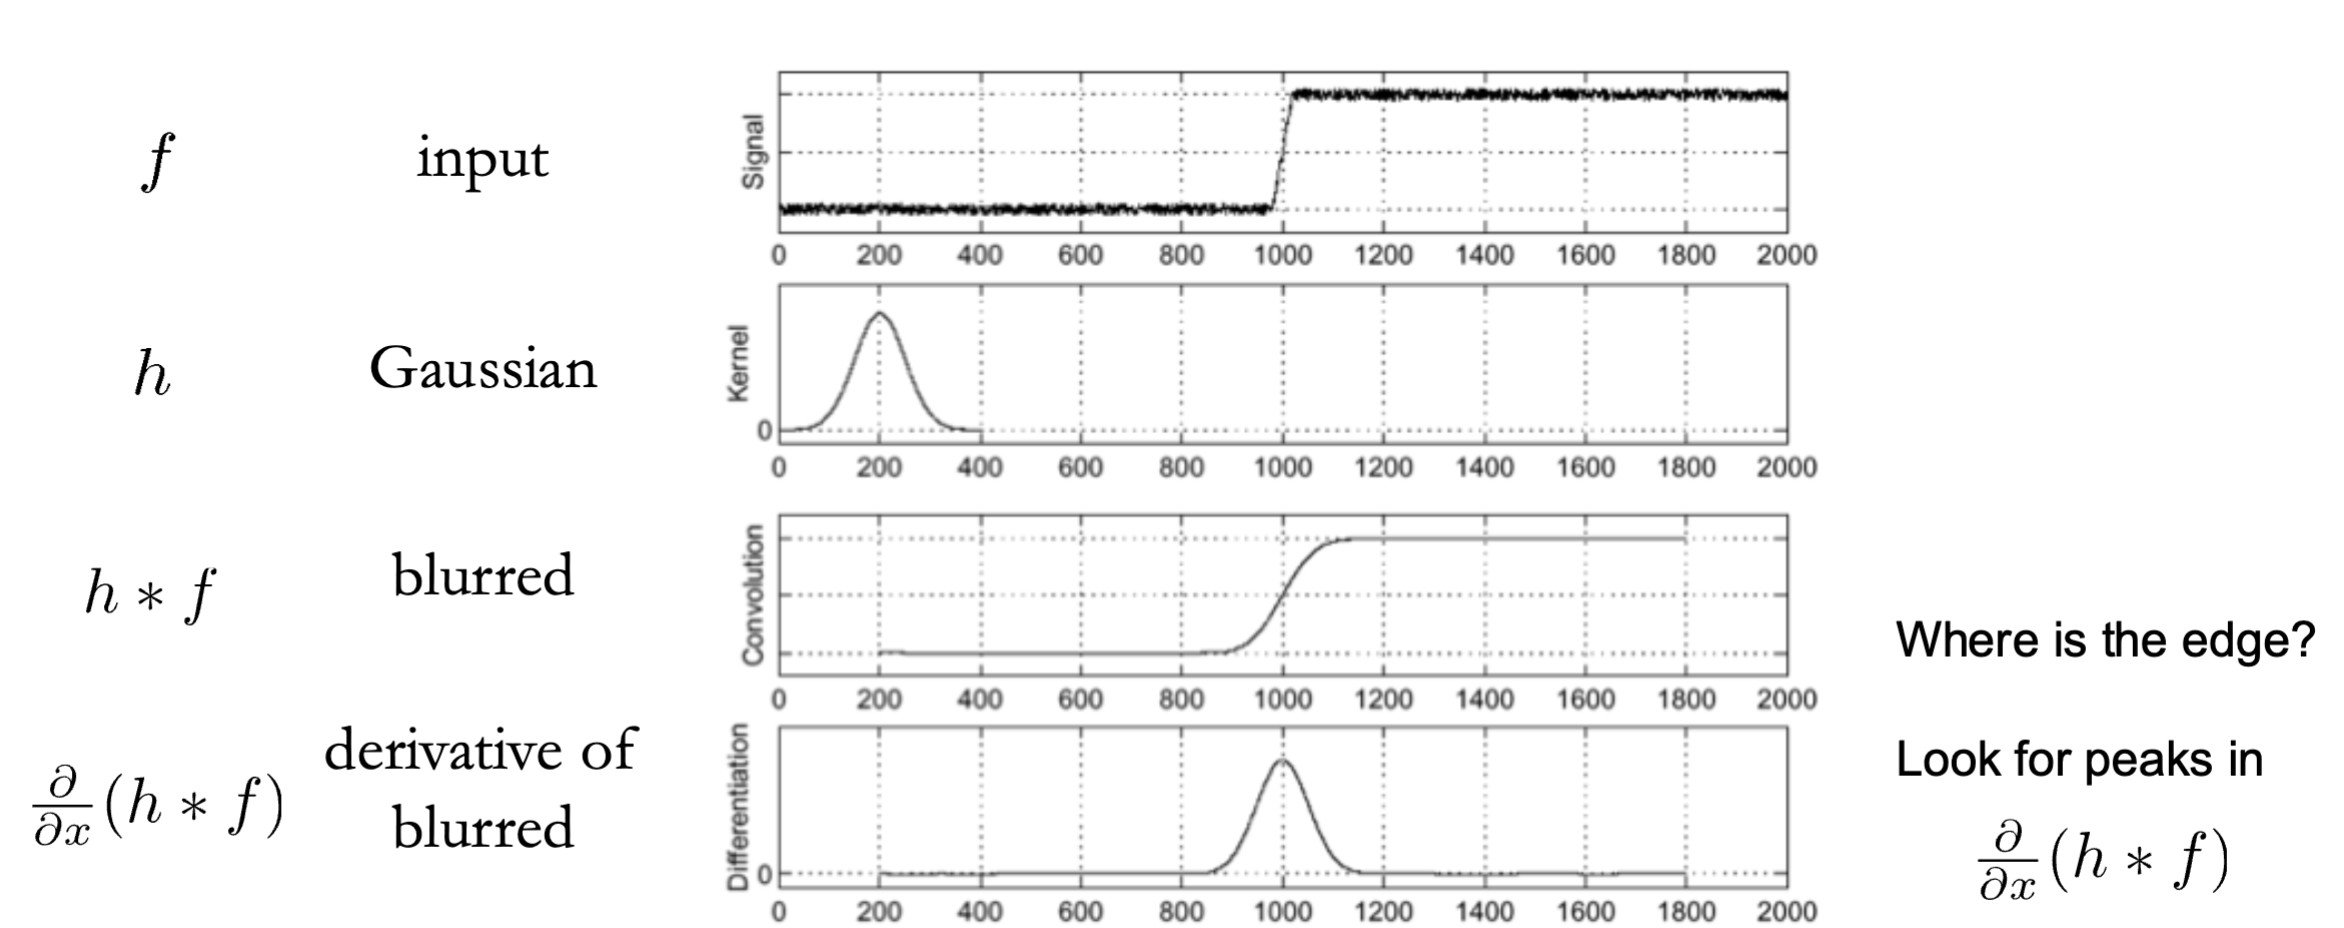
\includegraphics[width=0.75\linewidth]{blur.png}
\end{center}
Stronger Gaussian returns more high-frequency noise $\rightarrow$ spreads edge across larger region.

\textbf{Differentiation Property: } $\tfrac{\partial}{\partial x}(h * f) = \left(\tfrac{\partial}{\partial x}h\right) * f$ \\
Differentiation is a convolution operation:\\
$f * [1\;\;0\;\;{-1}]$ (x-direction) or $f * [1\;\;0\;\;{-1}]^T$ (y-direction)

\subsection{Laplacian Operator}
\begin{formulabox}
    Continuous: $\Delta f = \tfrac{\partial^2 f}{\partial x^2} + \tfrac{\partial^2 f}{\partial y^2}$ \\
    Discrete: $\nabla^2 f(x,y) = f(x{+}1,y)+f(x{-}1,y)+f(x,y{+}1)+f(x,y{-}1)-4f(x,y)$
\end{formulabox}


% ---------- Row 1: first-order finite difference ----------

% \begin{tabular}{@{}p{3.3cm}cc@{}}
% \mbox{$f'(x) = \displaystyle\lim_{h\to 0}\tfrac{f(x+0.5h)-f(x-0.5h)}{h}$} &
% $\longrightarrow$ &
% \begin{tabular}{@{}c@{}}1D derivative filter\\[3pt]\kernelrow{1}{0}{-1}\end{tabular}
% \\

% \mbox{$f''(x) = \displaystyle\lim_{h\to 0}\tfrac{f(x+h)-2f(x)+f(x-h)}{h^2}$} &
% $\longrightarrow$ &
% \begin{tabular}{@{}c@{}}1D Laplace filter\\[3pt]\kernelrow{1}{-2}{1}\end{tabular}
% \\

% {\tiny
% \begin{tabular}{@{}l@{}}
% $\nabla^2 f(x,y) = f(x{+}1,y){+}f(x{-}1,y)$\\
% $+f(x,y{+}1){+}f(x,y{-}1)-4f(x,y)$
% \end{tabular}} &
% $\longrightarrow$ &
% \begin{tabular}{@{}c@{}}2D Laplace filter\\[3pt]\kernelgrid{0}{1}{0}{1}{-4}{1}{0}{1}{0}\end{tabular}
% \end{tabular}


\textbf{Laplacian of Gaussian Filter}

\vspace{-1em}
\begin{center}
    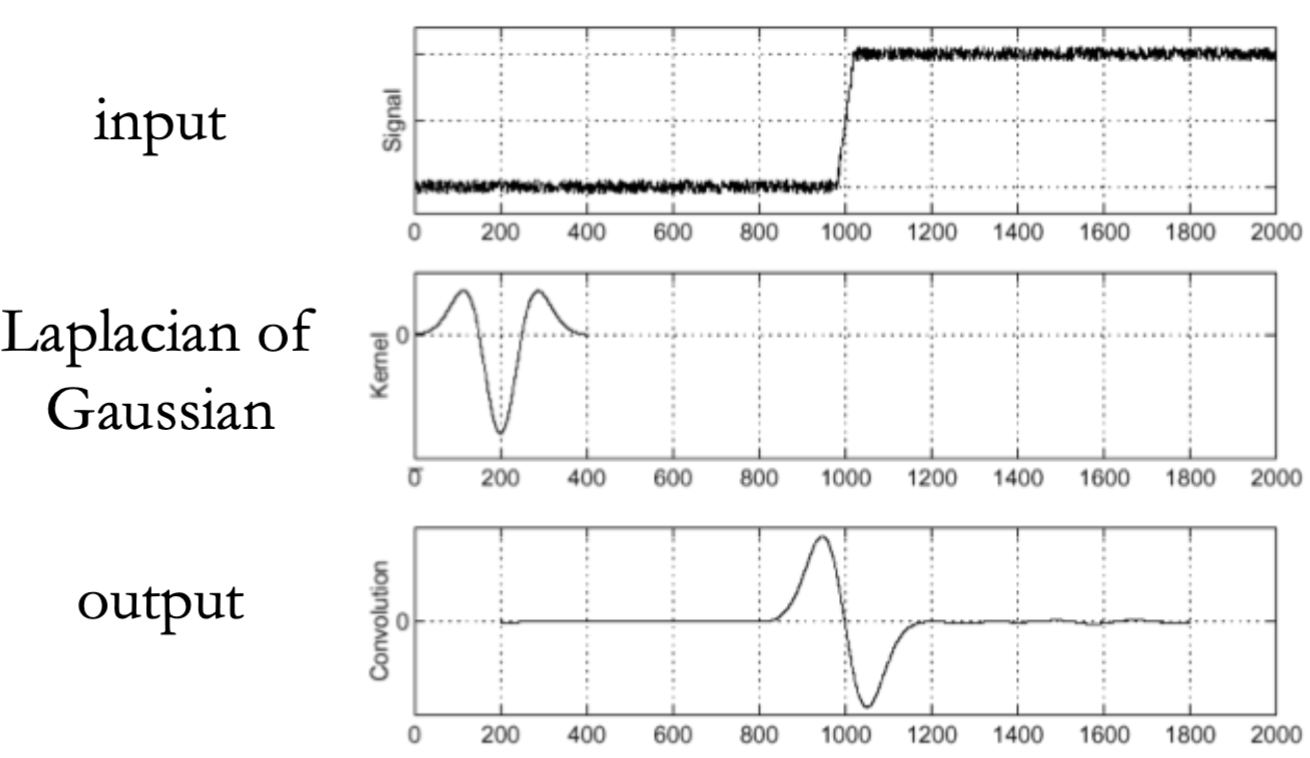
\includegraphics[width=0.75\linewidth]{laplacian.png}
\end{center}
\vspace{-1.5em}
\textbf{Zero crossings}. Localise edges more accurately but less convenient to use.

\subsection{Canny Edge Detector}
Deriv.\ of Gaussian $\rightarrow$ Grad.\ mag/orient. $\rightarrow$ NMS $\rightarrow$ Hysteresis thresh.\\
\textbf{Non-Maximum Suppression}: Only keep local maximums for edges (so edges will be one pixel wide.
\textit{Algorithm} Given magnitude map $M(x, y)$ and orientation map $\theta(x, y)$, for every $(x, y)$
\begin{enumerate}
    \item Find two neighbours in that direction according to the nearest angle ($+\theta, -\theta$)
    \item Interpolate the two neighbour values, with value $= x * (a - b) + b$, where $a, b$ are the two real neighbour pixel magnitudes, and $x$ is the fractional distance, $x = \tan(\theta mod 90)$
    \begin{center}
        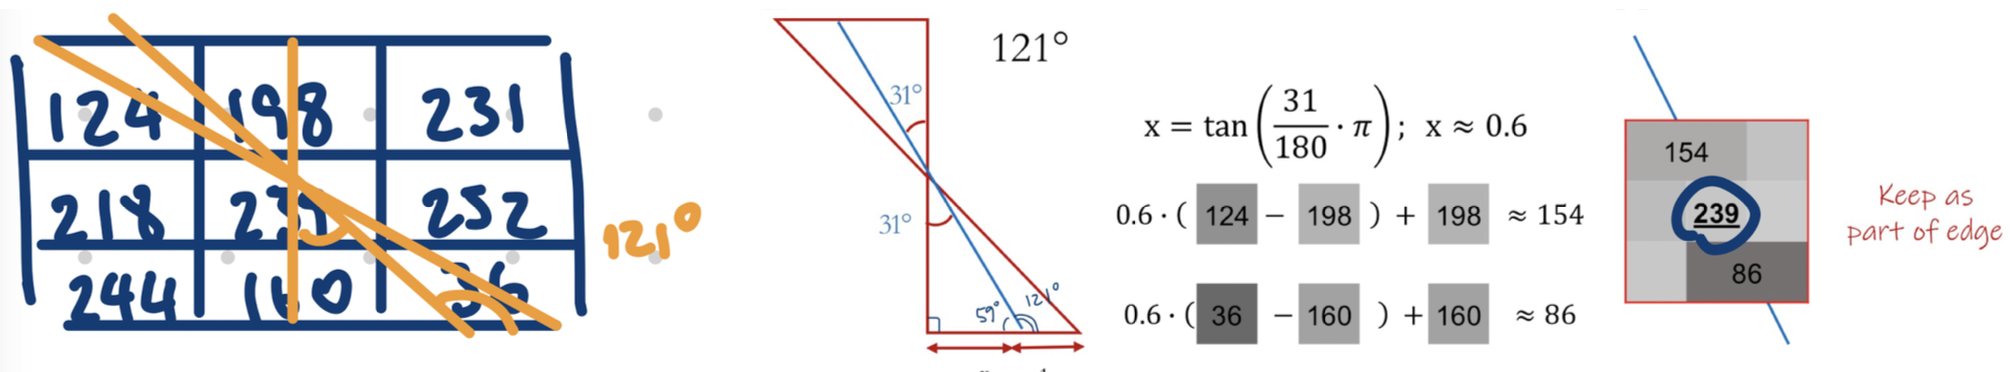
\includegraphics[width=0.75\linewidth]{interpolatenms.png}
    \end{center}
    \item Compare centre pixel to interpolated neighbours. 
    \begin{formulabox}
        If $M(x, y) \geq $ both neighbours: keep $M(x, y)$
        Else: suppress and set $M(x, y) = 0$
    \end{formulabox}
\end{enumerate}

\textbf{Hysterisis Thresholding}: Set two thresholds, $H$ to start edge curves, and $L$ to grow and link edges (if connected to boundary, mark said pixel as boundary) \\
\textit{Algorithm} $E_H$: set of all values passing $H$, $E_L$: set of all values passing $L$. Let $D = E_L - E_H$ (keep only edges of D connected to $E_H$) \\
Final image: $E_H \cup D'$

\textbf{Hough Transform}
\textit{Algorithm} Given magnitude map $M(x, y)$ and orientation map $\theta(x, y)$, for every $(x, y)$
\begin{enumerate}
    \item Quantise parameter space $(m, b)$ by picking a range and step size, then discretise.
    \item Initialise accumulator array $A(m, b)$. Set each $A(m, b) = 0,  \forall m, b$.
    \item $\forall (x_i, y_i), \forall m: b = x_im + y_i$. Increment $A(m, b) = A(m, b) + 1$
    \item Threshold and find local maxima of $A(m, b)$. $y = m^*x + b^*$
    \begin{formulabox}
        Use $x\cos\theta + y\sin\theta = \rho$ — finite parameters ($\theta \in [0,360]$) vs. unbounded gradient $m$
    \end{formulabox}
\end{enumerate}
Can be made more efficient by voting only near its measured gradient orientation.

\section*{Lecture 4 - Regions}
\sectionrule
\textbf{Filter banks}: collection of multiple filter kernels, where one filter kernel responds to one local pattern.
\textbf{Gabor Filter}: fix general math function with a range of parameters. Composed of sinuisoids and Gaussian envelope.

\begin{center}
    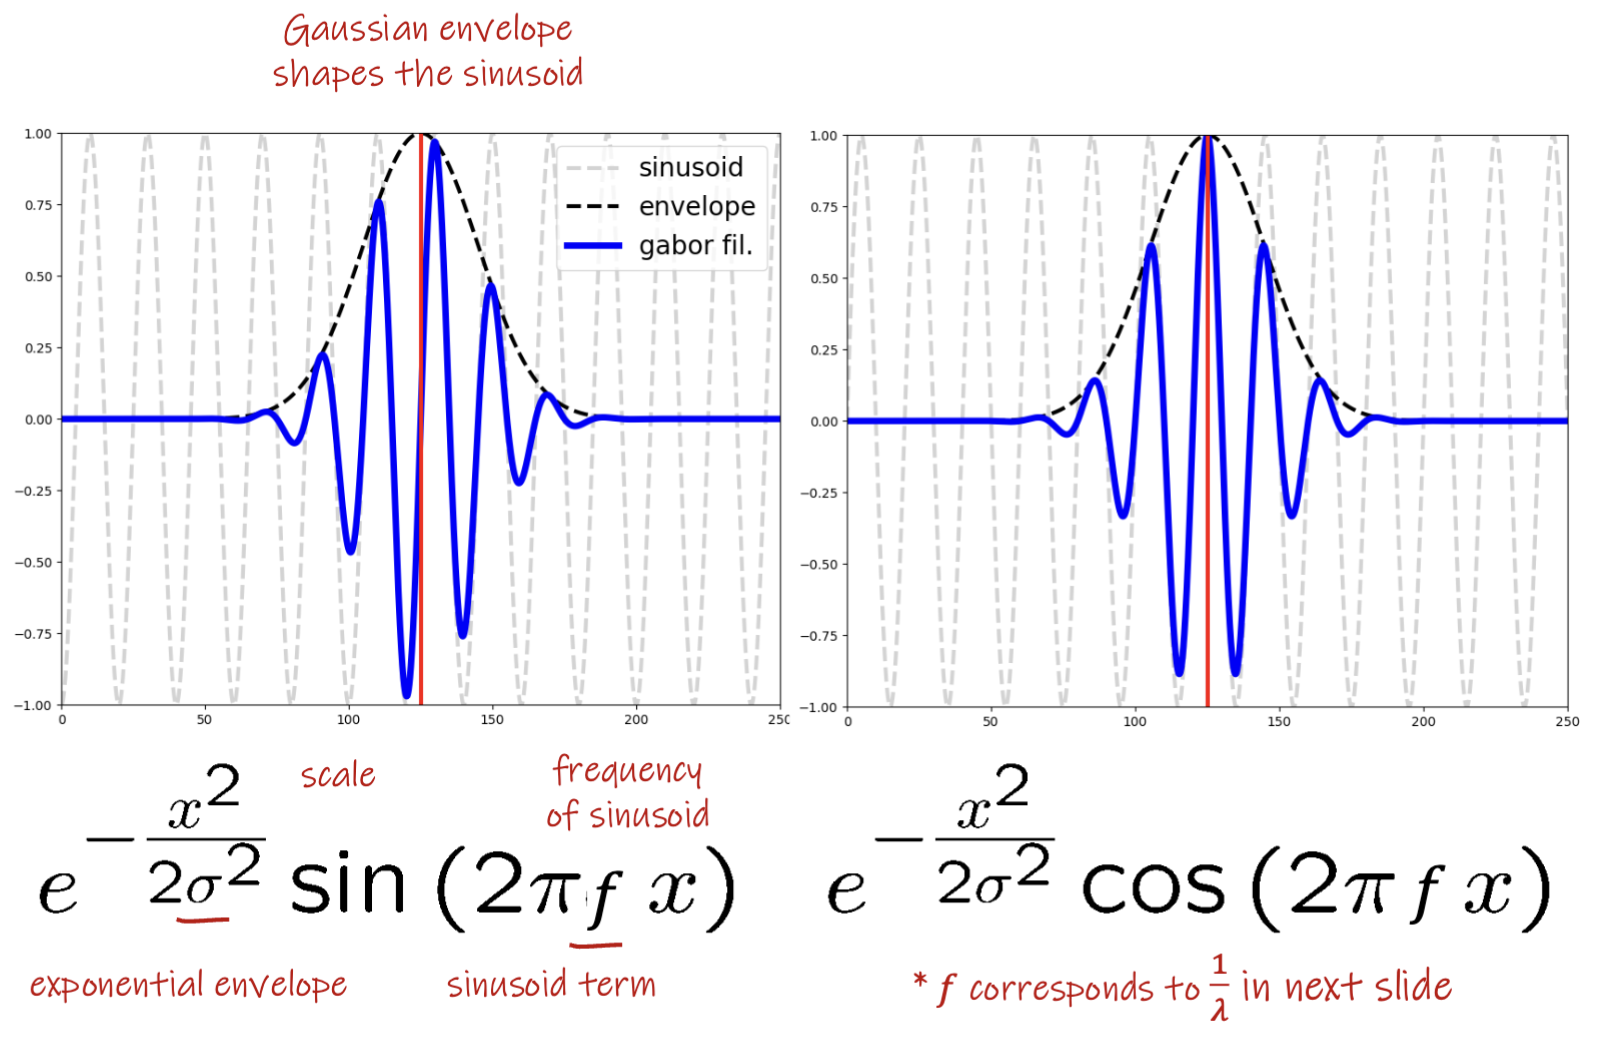
\includegraphics[width=0.75\linewidth]{gabor1d.png}
\end{center}
$f$: frequency selects spacing between waves; $\sigma$: scale determines size of region covered by Gaussian envelope. \\ 
\textit{2D Gabor formula}:
\[
\resizebox{\linewidth}{!}{$
f_{mn} = \underbrace{\frac{1}{2\pi\sigma^2}\exp\left[-\frac{m^2+\gamma^2 n^2}{2\sigma^2}\right]}_{\substack{\text{exponential (Gaussian) envelope} \\ \text{selects a local area}}}
\;\, \underbrace{\sin\left[\frac{2\pi(\cos[\omega]m+\sin[\omega]n)}{\lambda}+\phi\right]}_{\substack{\text{2D-Sinusoid} \\ \text{selects orientation and frequency}}}
$}
\]
$\omega$ -- orientation of sinusoid in 2D \\
$\lambda$ -- wavelength of sinusoid (inversely proportional to $f$) \\
$\phi$ -- phase of sinusoid; shift from center of kernel
$\gamma$ -- aspect ratio of envelope coverage ($\gamma = 1$ means circular, otherwise elliptical) \\
$\sigma$ -- rate of decay of exponential envelope

\subsection{Multi-Scale Reasoning}
\textbf{Smoothing} suppresses details, which we want to ignore variations in smaller distances to focus on larger structure.
\textit{Gaussian image pyramid} $\rightarrow$ progressively blur then downsample at fixed stride or downsampling rate. \\
We should smooth before downsampling to prevent aliasing (high-frequency can mask as low frequency, ringing).

\textbf{Scale selection} Measure responses on multiple scales. Choose maximum filter size that matches structure size to detect structures. 

\textbf{Single vs Multi-scale Representation} Given $r_i, \rho_i$ corresponding to response and scale at $i$. \\
\textit{Single scale}: $r = [r_1, r_2, ..., r_k]$ \\
\textit{Multi-scale: } $r = [r_1^{\rho_1}, r_2^{\rho_1}, ..., r_k^{\rho_1}, r_1^{\rho_2}, ..., r_k^{\rho_2}]$.

\subsection{Textures}
\textit{Textures} occur over an area. To detect, group pixels by region $\Omega$ and average filter responses over region.
\begin{enumerate}
    \item $r(x, y) = [r_1(x, y), r_2(x, y), ..., r_k(x, y)]$ Run $k$ different filters to get $k$ responses.
    \item $t_k(\Omega) = \tfrac{1}{|\Omega|}\sum|r_k(x, y)|$. Take absolute value of every pixel's response to filter $k$ in region $\Omega$ and sum. Divide pixels by $|\Omega|$ for average. \\
    $t_k(\Omega)$ is a pooled response of filter $k$ across $\Omega$
    \item $t(\Omega) = [t_1(\Omega), t_2(\Omega),..., t_k(\Omega)]^T$
\end{enumerate}

\begin{formulabox}
    To compare textures, $D(\Omega_A, \Omega_B) = ||t(\Omega_a) - t(\Omega_a)||$, i.e. $D$ is the Euclidean distance.
\end{formulabox}

\textit{Classifiers}
\begin{enumerate}
    \item Nearest Neighbour Classifier: $i^* = \arg\min_i ||t(\Omega)-t(\Omega_i)||$ where $\hat{c} = y_{i^*}$
    \item Nearest Class Mean: $\mu_c = \tfrac{1}{N_i}\sum{i:y_i=c}{t(\Omega_c)}$ where $\hat{c}(\Omega) = \arg\min ||t(\Omega)-\mu_c||$
\end{enumerate}
\vspace{-1.5em}

\begin{center}
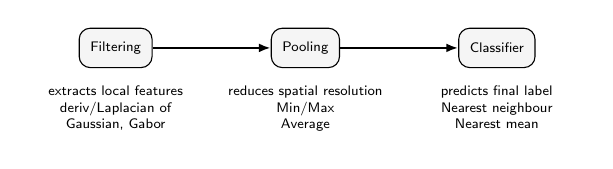
\begin{tikzpicture}[
    box/.style={draw, rounded corners, fill=gray!8, minimum height=0.5cm,
                align=center, font=\tiny, inner sep=4pt},
    arr/.style={-{Latex[length=1.5mm]}, thick},
    caption/.style={font=\tiny, align=center, text width=2cm},
    every node/.append style={font=\tiny}
  ]
  \node[box] (filter) {Filtering};
  \node[box, right=1.5cm of filter]  (pool) {Pooling};
  \node[box, right=1.5cm of pool]  (class)   {Classifier};

  \draw[arr] (filter) -- (pool) ;
  \draw[arr] (pool) -- (class);

  \node[caption, below=0.1cm of filter] {extracts local features \\ deriv/Laplacian of \\ Gaussian, Gabor};
  \node[caption, below=0.1cm of pool]  {reduces spatial resolution \\ Min/Max \\ Average};
  \node[caption, below=0.1cm of class]  {predicts final label \\ Nearest neighbour \\ Nearest mean};
\end{tikzpicture}
\end{center}
\vspace{-1.5em}

\section*{Topic 5 - CNNs}
\sectionrule
\textbf{Receptive field}: set of image pixels an intermediate output pixel depends on. \\
\textit{Recursive formula} (per layer $l$, with kernel $k_l$, stride $s_l$):
$r_l = r_{l-1} + (k_l - 1)\, j_{l-1}, \qquad j_l = j_{l-1}\, s_l$
\text{base case: } $r_0 = 1,\; j_0 = 1$

\textbf{Training:} \quad \colorbox{red!10}{Training Images} $\rightarrow$ Image Features $\rightarrow$ Training with Labels $\rightarrow$ Learned Classifier

\textbf{Testing:} \quad Test Image $\rightarrow$ Image Features $\rightarrow$ Learned Classifier $\rightarrow$ Prediction

\textbf{Stages of Classifier}
\begin{center}
    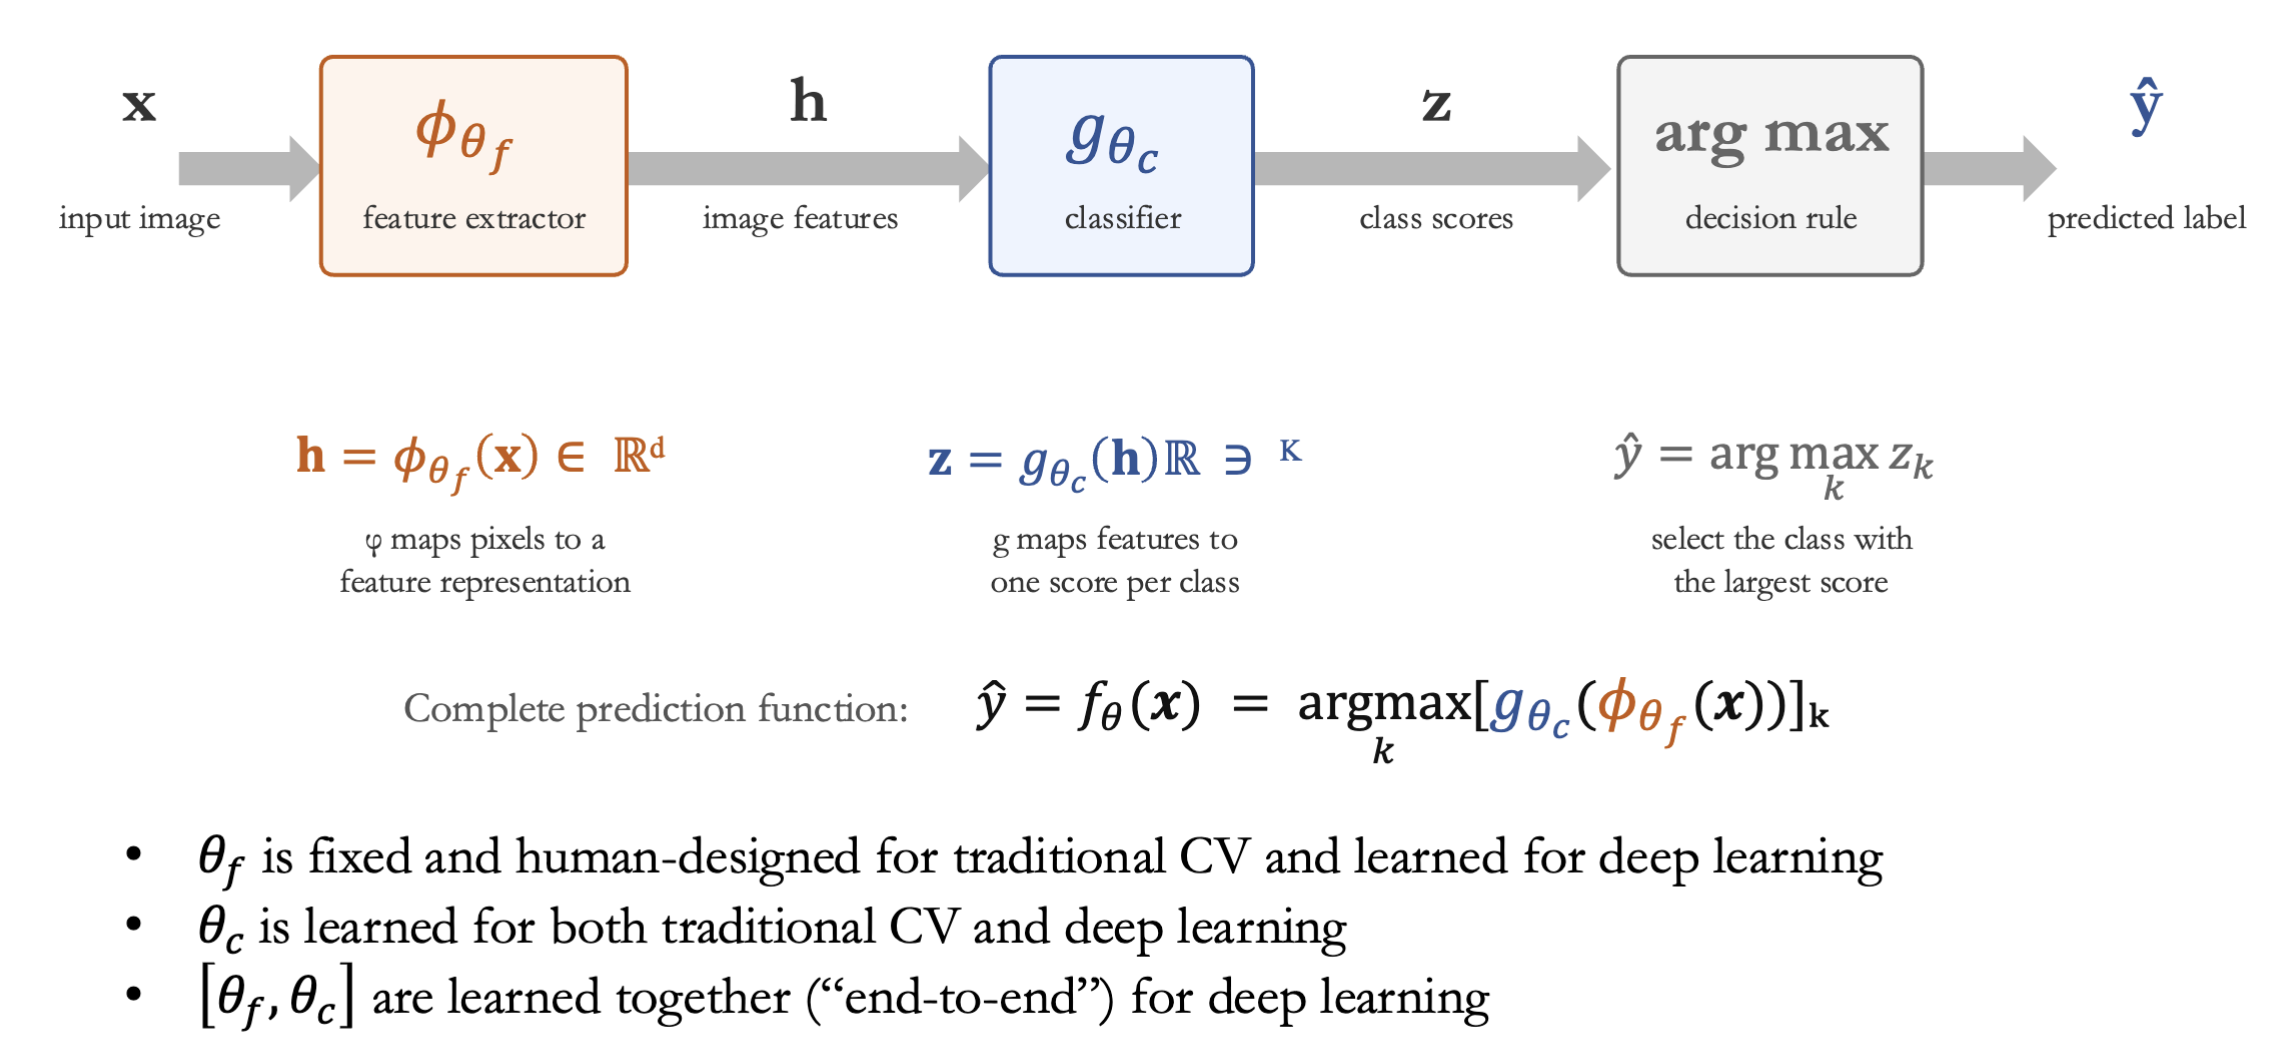
\includegraphics[width=0.9\linewidth]{classifierstage.png}
\end{center}

\textbf{Perceptron}
\begin{center}
    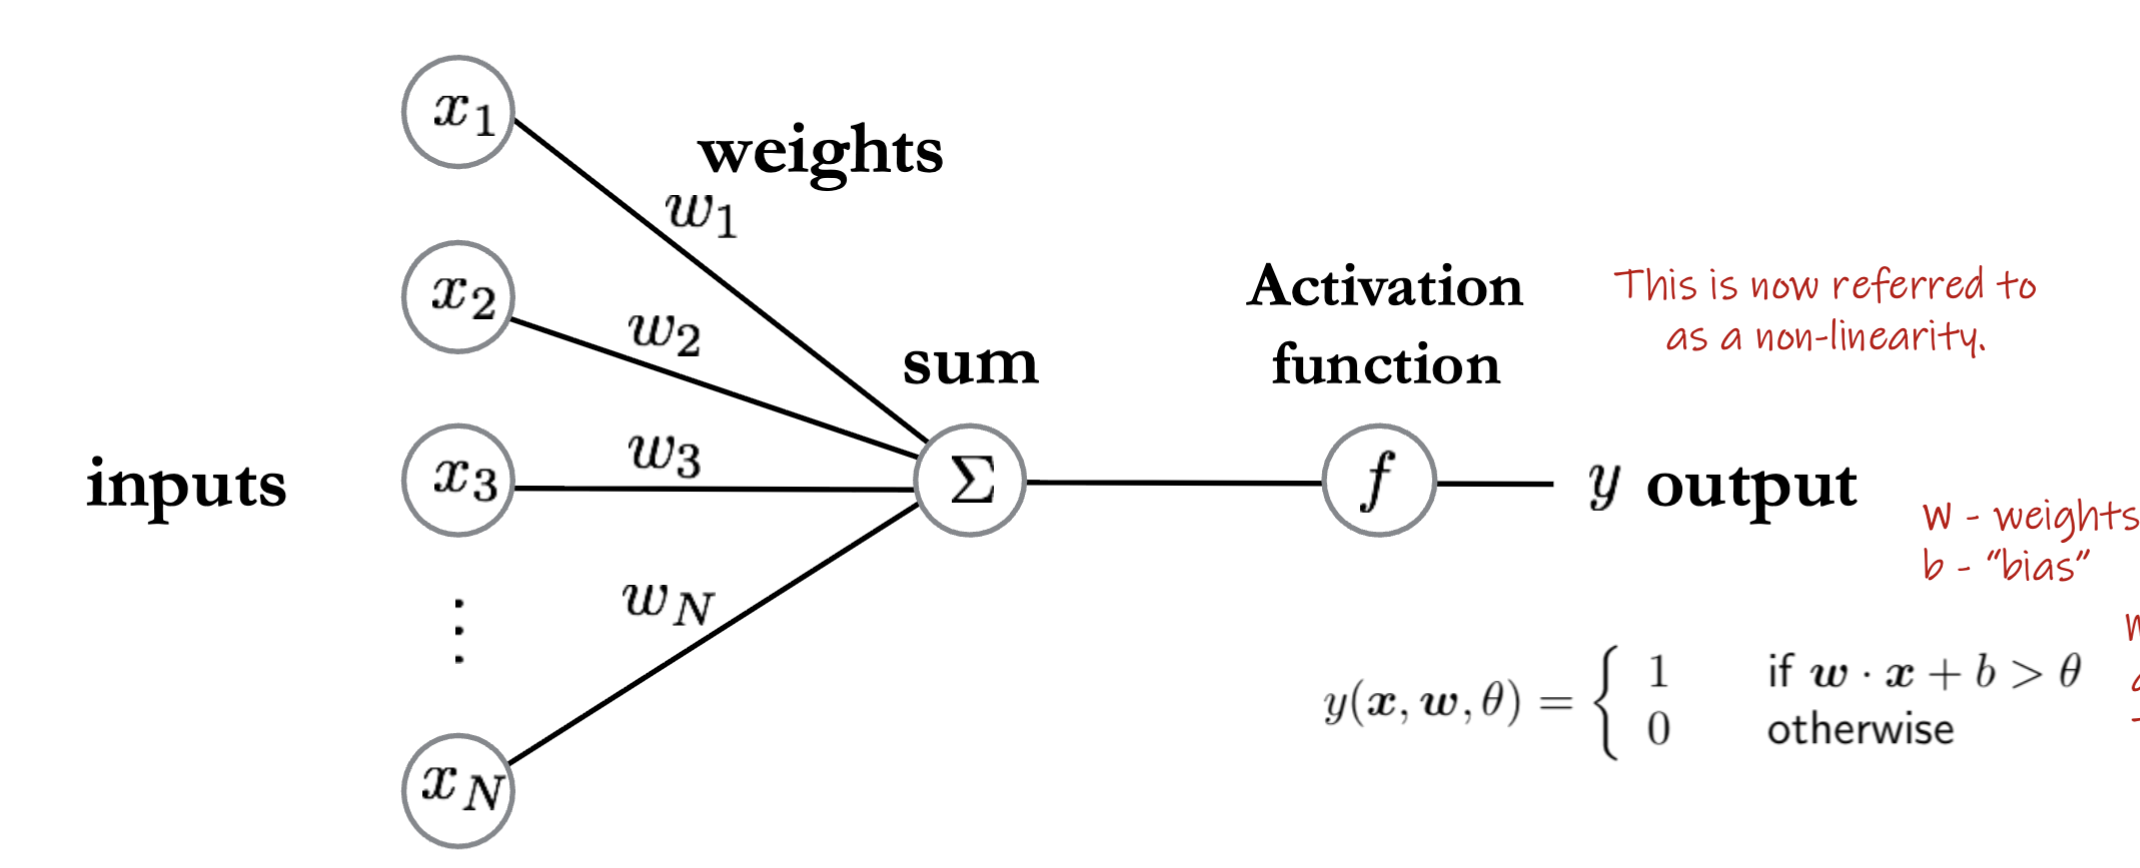
\includegraphics[width=0.75\linewidth]{perceptron.png}
\end{center}
No of learnable parameters = weights (edges) + perceptrons (neurons). \\
Neurons are total of all possible output nodes (all layers except input). We add perceptrons as bias terms.

\textbf{MLP Formalism} \\
\noindent\textbf{Input:} \quad
$\mathbf{a}^{(0)} = \mathbf{u}$; 
\hfill \parbox{5.5cm}{\footnotesize $\mathbf{u}$: input feature vector}

\noindent\textbf{Hidden layers:}
\[
\mbox{$\mathbf{a}^{(\ell)} = \sigma\Big(W^{(\ell)}\mathbf{a}^{(\ell-1)} + \mathbf{b}^{(\ell)}\Big), \; \ell = 1,\dots,L-1$}
\]
\footnotesize
$\boldsymbol{a}^{(\ell)}$: representation in layer $\ell$. \\
$W^{(\ell)}$: weights in layer $\ell$. \\
$\boldsymbol{b}^{(\ell)}$: biases in layer $\ell$. \\
$\sigma$: non-linear activation function

\noindent\textbf{Output}\textbf{ layer:} \quad
$\mbox{$\mathbf{z} = \mathbf{a}^{(L)} = W^{(L)}\mathbf{a}^{(L-1)} + \mathbf{b}^{(L)}$}$

\subsection{Convolution}
\begin{formulabox}
    No of learnable parameters: $$k^2 \cdot C_{in} \cdot C_{out} + C_{out}$$
\end{formulabox}
\textbf{Strided}. Downsample each feature map. Reduce spatial resolution.
\textbf{Dilated}. Enlarge receptive field without adding params or reducing resolution. 
\begin{formulabox}
    $H_{output} = \left\lfloor \frac{H_{input} + 2P - D(K-1) - 1}{S} \right\rfloor + 1$
\end{formulabox}

\textbf{Logits}: unrestricted real-value scales $\rightarrow$ convert into probability distribution using softmax.

\subsection{Loss functions}
\begin{center}
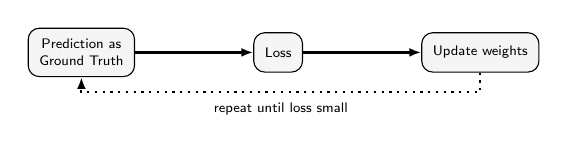
\begin{tikzpicture}[
    box/.style={draw, rounded corners, fill=gray!8, minimum height=0.5cm,
                align=center, font=\tiny, inner sep=4pt},
    arr/.style={-{Latex[length=1.5mm]}, thick},
    darr/.style={-{Latex[length=1.5mm]}, thick, dotted},
    every node/.append style={font=\tiny}
  ]
  \node[box] (pred) {Prediction as \\ Ground Truth};
  \node[box, right=1.5cm of pred]  (loss) {Loss};
  \node[box, right=1.5cm of loss]  (update) {Update weights};

  \draw[arr] (pred) -- (loss) ;
  \draw[arr] (loss) -- (update);

  \draw[darr] (update.south) -- ++(0,-0.25cm) -| node[below, pos=0.25, font=\tiny] {repeat until loss small} (pred.south);
\end{tikzpicture}
\end{center}
\vspace{-1.5em}

\textit{Examples}
\begin{enumerate}
    \item Localisation loss: $L_{\text{loc}} = (\hat{x}-x)^2 + (\hat{y}-y)^2$. Distance-based, naturally continuous.
    \item $L_{0/1}(\hat{y}, y) =
        \begin{cases}
        0, & \hat{y} = y \quad \text{(correct)} \\
        1, & \hat{y} \neq y \quad \text{(wrong)}
        \end{cases}
    $. Discrete
    \item Cross-entropy loss: $L_{\text{CE}} = -\log(p_y)$. Continuous — softly penalizes low confidence in the correct class
\end{enumerate}

\subsection{Object Detection}
\textbf{Window-based}: \quad Build/train model $\rightarrow$ Generate candidate windows $\rightarrow$ Score candidates $\rightarrow$ Resolve detections with NMS. \\
\textit{Performance Evaluation} Area of Overlap Measure $AO(B_{gt}, B_p) = \frac{|B_{gt} \cap B_p|}{|B_{gt} \cup B_p|}$

\textbf{mAP (mean Average Precision):} standard object-detection metric, 0--1 or 0--100\%. We want high precision (few false positives) and high recall (few false negatives).

\begin{itemize}
    \item AP$(c,\tau)$ = area under precision--recall curve (class $c$, IoU $\geq \tau$)
    \item mAP$(\tau)$ = mean AP across classes
\end{itemize}
\vspace{-1em}

\[
\text{AP}(c,\tau) = \int_0^1 p(r)\,dr \qquad \text{mAP}(\tau) = \frac{1}{|C|}\sum_{c \in C} \text{AP}(c,\tau)
\]

\subsection{CNN-Based Object Detection}

\section*{Topic 6 - Segmentation}
\sectionrule
Separation of images into regions/objects. \\
\textbf{Semantic}: each pixel has a class label. Identify foreground and background. \\ 
\textbf{Instance}: Each pixel has an object it belongs to.
\textbf{Panoptic}: Combine semantic and instance.

\textit{Pixel affinity}: evidence that makes two pixels belong to the same region (color, texture, etc.).

\textbf{k-Means Clustering}: Iteratively re-assign points to nearest cluster center
\begin{enumerate}
    \item Randomly initialize the cluster centers $c_1, \ldots, c_K$
    \item For each point $p_i$, find the closest $c_j$ to put $p_i$ in
    \item Set $c_j$ to be mean of points in cluster $j$
    \item Repeat, if $c_j$ have changed up to some threshold
\end{enumerate}
\begin{itemize}
    \item Pros: Simple, Converges to local min.
    \item Cons: Setting $K$, Sensitive to initial centers (Since k-means converges to local min.), Sensitive to outliers (Can add more clusters), Assumes spherical clusters
\end{itemize}
\textbf{Simple Linear Iterative Clustering (SLIC)}
\begin{itemize}
    \item \textit{Superpixel}: Group of pixels that share common traits. Compact and meaningfyl representation.
    \item No of pixels: $n_{tp}$; Target no of superpixels: $n_{sp}$
    \item Initial width of each superpixel: $s = \sqrt{n_{tp} / n_{sp}}$
    \item Features: $z = [r,g,b,x,y]$
    \item Color distance: $d_c = || \langle r_j,g_j,b_j \rangle - \langle r_i,g_i,b_i \rangle ||$
    \item Spatial distance: $d_s = || \langle x_j,y_j \rangle - \langle x_i,y_i \rangle ||$
    \item $d_{cm}$ and $d_{sm}=s$ set as max. expected values of $d_c$ and $d_s$ respectively
    \item $D = \sqrt{(\frac{d_c}{d_{cm}})^2+(\frac{d_s}{d_{sm}})^2} = \sqrt{d_c^2 + (\frac{d_s}{s})^2 c^2}$
\end{itemize}
\begin{enumerate}
    \item Split img. into grid of size $s \times s$. Set cluster centers as lowest gradient position in $3 \times 3$ neighborhood from superpixel center. 
    \item For each cluster center, check distance to all pixels within $2s \times 2s$ neighborhood. Assign pixels to closest checked center.
    \item Update cluster centers using mean; repeat until converged (Same as k-Means)
    \item Optional: Replace superpixel region by average value to create stained glass effect
\end{enumerate}
\begin{itemize}
    \item Modification of k-Means: Not random initialization, Compute pixel's distance only to closest set of centers
\end{itemize}
\textbf{Mean-Shift Clustering}: Find local density maxima in feature space 
\begin{itemize}
    \item \textit{Attraction basin}: {Region in feature space for which all trajectories of centroids lead to same mode}
    \item \textit{Cluster}: {All data points in attraction basin of a mode}
\end{itemize}
\begin{enumerate}
    \item For each data point:
    \begin{enumerate}
        \item Define window around and get centroid
        \item Shift window to centroid
        \item Repeat until window centroid stops moving
    \end{enumerate}
\end{enumerate}
\begin{itemize}
    \item Segmentation with Mean Shift: Do mean shift and merge pixels in same attraction basin
    \item Choosing window size: Trial and error, Sample points and use avg. dist. to knn. (Num. of neighbors needs to be large enough to ensure increase in density)
    \begin{itemize}
        \item Larger window size $\rightarrow$ Fewer clusters
    \end{itemize}
    \item Pros: No assumptions on cluster shape, 1 parameter, Finds variable num. of modes (vs. specified $k$ in k-Means), Robust to outliers
    \item Cons: Choosing $h$, Slow, Scales poorly with feature space dimension
    \item Optimizations:
    \begin{itemize}
        \item After each run of mean shift, assign all points within radius $r$ of end point to same cluster
        \item Assign points in radius $c < r$ of search path to mode
    \end{itemize}
\end{itemize}

\end{multicols}

\end{document}